\begin{center}
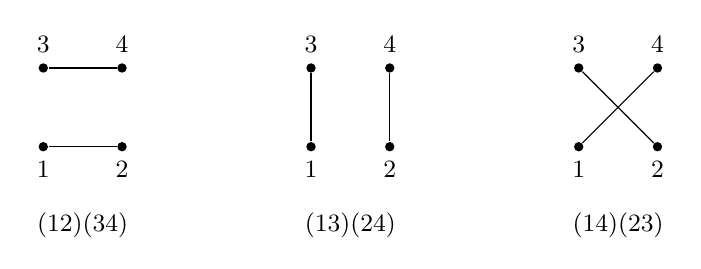
\begin{tikzpicture}[scale=1, every node/.style={font=\small}]
\tikzset{
  v/.style={circle, fill, inner sep=1.2pt},
  lab/.style={inner sep=1pt},
  bub/.style={circle, draw, inner sep=1.5pt}
}

% --- pairing (12)(34) ---
\begin{scope}[xshift=0cm]
  \node[v,label=below:$1$] (a1) at (0,0) {};
  \node[v,label=below:$2$] (a2) at (1,0) {};
  \node[v,label=above:$3$] (a3) at (0,1) {};
  \node[v,label=above:$4$] (a4) at (1,1) {};
  \draw (a1)--(a2); \draw (a3)--(a4);
  \node[lab] at (0.5,-1) {$(12)(34)$};
\end{scope}

% --- pairing (13)(24) ---
\begin{scope}[xshift=3.4cm]
  \node[v,label=below:$1$] (b1) at (0,0) {};
  \node[v,label=below:$2$] (b2) at (1,0) {};
  \node[v,label=above:$3$] (b3) at (0,1) {};
  \node[v,label=above:$4$] (b4) at (1,1) {};
  \draw (b1)--(b3); \draw (b2)--(b4);
  \node[lab] at (0.5,-1) {$(13)(24)$};
\end{scope}

% --- pairing (14)(23) ---
\begin{scope}[xshift=6.8cm]
  \node[v,label=below:$1$] (c1) at (0,0) {};
  \node[v,label=below:$2$] (c2) at (1,0) {};
  \node[v,label=above:$3$] (c3) at (0,1) {};
  \node[v,label=above:$4$] (c4) at (1,1) {};
  \draw (c1)--(c4); \draw (c2)--(c3);
  \node[lab] at (0.5,-1) {$(14)(23)$};
\end{scope}
\end{tikzpicture}
\end{center}
